\documentclass[10pt]{article}
\usepackage{graphicx} % Required for inserting images
\usepackage[a4paper, total={6in, 8in}, margin=.8in]{geometry}
\usepackage{amsmath}
\usepackage{amssymb}
\newtheorem{theorem}{Theorem}
\newtheorem{definition}{Definition}
\title{Chengcheng Rotation Week Update}
\author{Lane Lewis}
\date{June 2023}

\begin{document}

\maketitle
\section{Week Overviews}
\subsection{Week 1}
\begin{itemize}
    \item Built the single region network
    \item Replicated figure 2 of 'The Dynamical Regime of Sensory Cortex: Stable Dynamics around a Single Stimulus-Tuned Attractor Account for Patterns of Noise Variability'
    \item Started building the two region network. Made a mistake in the input noise, the standard deviation was much larger than it should be. Originally had placed the same input into both regions instead of only region 1.
\end{itemize}
\subsection{Week 2}
\begin{itemize}
    \item Corrected the input noise and changed to a single input into region 1 instead of both regions. 
    \item Fixed the feedback weights to 0 and modified the feedforward weights to minimize the l2 norm between the region 1 and region 2 population rates. Plotted the best fit network across changing input over time.
    \item Using the feedforward weights that best balanced the rates between the two regions, the feedback weight from region 2 E to region 1 E was fixed to 1 and the EI ratio was modified from region 2 to region 1. Plotted the EI ratio's effect on the mean voltage across input strengths as well as the standard deviation across the input strengths.
\end{itemize}
\section{Notation}
The notation used was modified from 'the Dynamical Regime of Sensory Cortex: Stable Dynamics around a Single
Stimulus-Tuned Attractor Account for Patterns of Noise Variability'. Unless noted otherwise the weight from neuron/population i $\to$ j is denoted by $W_{ji}$\\
\textbf{Within Region 1 Variables/Constraints}:\\
\hspace*{1cm} Weights: $W_{1E1E}=1.25,W_{1E1I}=.65,W_{1IE1}=1.2,W_{1I1I}=.5$\\
\hspace*{1cm} Time Constants: $\tau_{1E} = 20$ms,$\tau_{1I}=10$ms\\
\hspace*{1cm} Private Noise: $\sigma_{1E} = .2, \sigma_{1I} = .1$\\
\hspace*{1cm} Input: $h_{1E} = h_{1I}$\\
\hspace*{1cm} Initial Conditions: $V^{(0)}_{1E} = V^{(0)}_{1I} = -70$\\
\textbf{Within Region 2 Variables/Constraints}:\\
\hspace*{1cm} Weights: 
$W_{2E2E}=1.25,W_{2E2I}=.65,W_{2I2E}=1.2,W_{2I2I}=.5$\\
\hspace*{1cm} Time Constants: $\tau_{2E}=20$ms,$\tau_{2I}=10$ms\\
\hspace*{1cm} Private Noise: $\sigma_{2E} = .2, \sigma_{2I} = .1$\\
\hspace*{1cm} Input: $h_{2E} = h_{2I} = 0$\\
\hspace*{1cm} Initial Conditions: $V^{(0)}_{2E}=V^{(0)}_{2I}=-70$\\
\textbf{Across Region Variables/Constraints}:\\
\hspace*{1cm} Weights: $W_{2E1I} = W_{1I2I} = W_{1E2I}=W_{2I1I} = 0, W_{2E1E},W_{2I1E},W_{1E2E},W_{1I2E}$\\
\textbf{Noise Parameters}:\\
\hspace*{1cm} Time Constants: $\tau_{Noise} = 50$ms\\
\hspace*{1cm} Initial Conditions: $\boldsymbol \eta_0 = \boldsymbol 0$
\begin{figure}
    \centering
    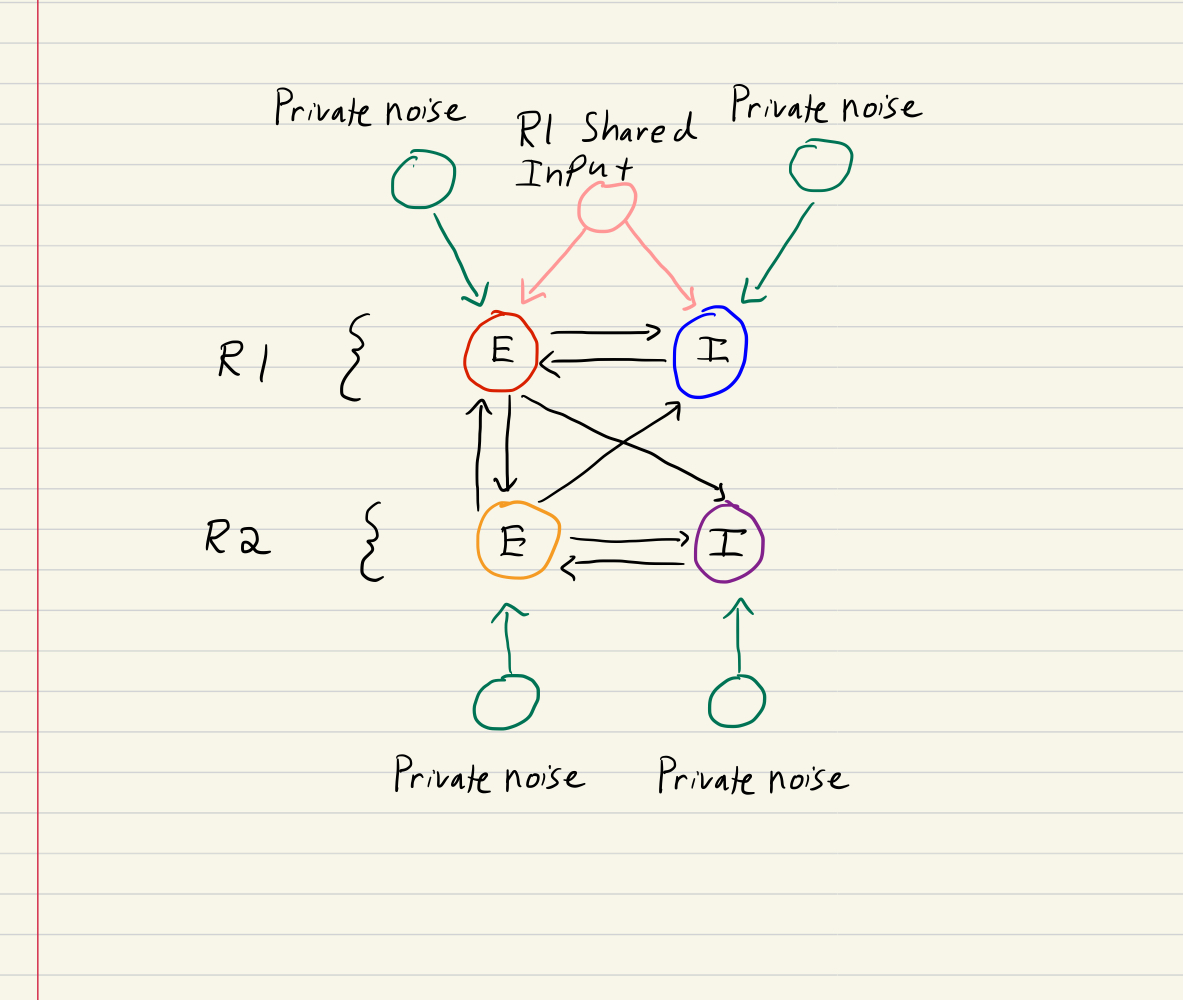
\includegraphics[scale=.2]{model.jpg}
    \caption{Model graph setup used for two region network}
\end{figure}
\section{Single Region Simulation}
\subsection{Description}
For the single region plots, an euler integral approximation was used for simulation. For plot 1 panel a, a simulation was run continuously where the input $h_1$ to region 1 was increased over time in steps from 2 to 5 to 15. Each time step was 2.5s with a division of 25000. The initial conditions were that the initial voltage for all were set to -70. For plot 1 panel b, the input was increased in steps from 0 to 20 where each input section was run for 7.5 seconds with a division of 75000. The mean and standard deviation were calculated across a single run within the respective stimulus input windows.
\subsection{Results}
The graphs closely mimic figure 2 from the paper indicating that the network was set up correctly. There is the interesting peak in variability when the input current is 2.
\begin{figure}[h]
    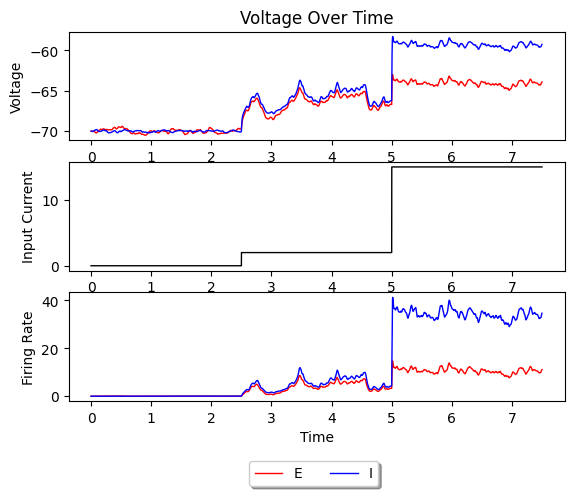
\includegraphics[scale=.5]{oneRegion/threeStepVoltage.png}
    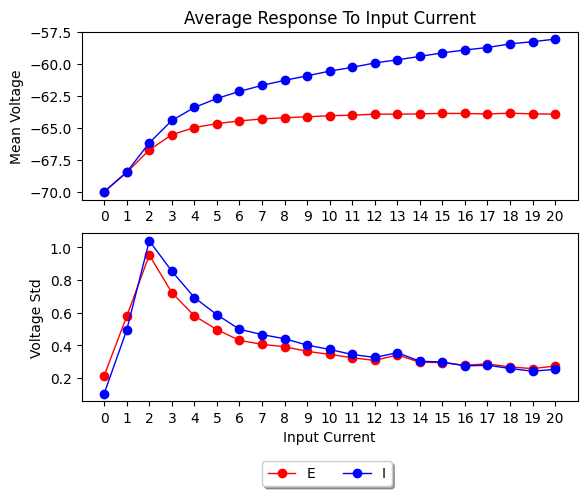
\includegraphics[scale=.5]{oneRegion/manyStepVariablility.png}
    \caption{Replicating Figure 2 of 'The Dynamical Regime of Sensory Cortex: Stable Dynamics around a Single Stimulus-Tuned Attractor Account for Patterns of Noise Variability' Left: Shared variability changes as a function of the input. Right: The variability peaks at an input of 2 }
\end{figure}
\section{Two Region Simulation Feedforward Balancing}
\subsection{Description}
For this simulation, the feedback weights $W_{1E2E}=W_{1E2I}=0$. The feedforward weights were run over the cartesian product of $W_{2E1E} \in [.5,.6,..., 1.5]$,$W_{2I1E} \in [.5, .6,...,1.5]$. The input was increased over time in steps of 1 from 0 to 20 where each step was 2.5s with 25000 divisions. Let the simulation output rate be the matrix $\boldsymbol R$ with columns being populations and rows being time. The loss function chosen was $L(\boldsymbol R) = ||\boldsymbol R_{1E} - \boldsymbol R_{2E} ||_2^2 + ||\boldsymbol R_{1I} -\boldsymbol R_{2I}||^2_2$. The simulation with the smallest average loss across 5 runs was $W_{2E1E} = 1.1, W_{2I1E} = 1.1$.
\subsection{Results}
There wasn't a perfect fit network that matched the mean rate exactly across all inputs. However, the best fit network did do fairly well, it was tight across a large set of the parameter space, particularly in the middle. The inhibitory currents were the most seperated. We still see a peak in variability around 2 across the network.
\begin{figure}[h]
    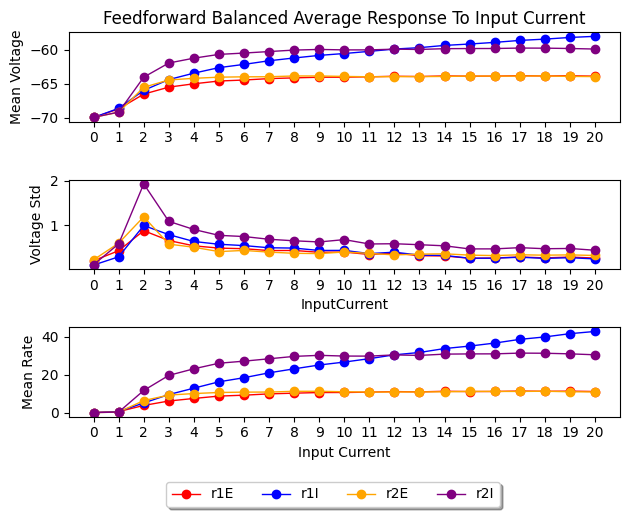
\includegraphics[scale=.5]{twoRegion/feedforwardAverageResponse.png}
    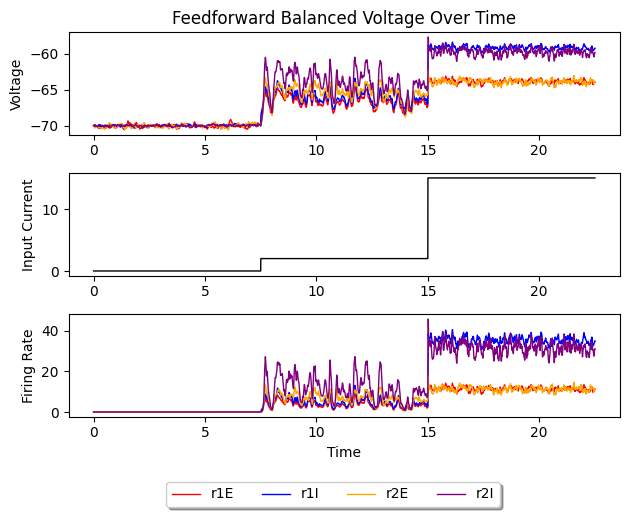
\includegraphics[scale=.5]{twoRegion/feedforwardVoltageOverTime.png}
    \caption{Best fit feedforward weights $W_{2E1E} = 1.1, W_{2E1I}=1.1$ for zero feedback weights for obtaining a region balanced firing rate. Left: Example voltage over time across inputs 0,2, and 15 for best fit network}
\end{figure}
\section{Two Region Simulation Feedback EI Ratio}
\subsection{Description}
For this simulation, the feedforward weights were fixed using the parameters found in the feedforward balancing simulation: $W_{2E1E} = W_{2I1E} = 1.1$. The feedback weight from excitatory to excitatory was fixed, $W_{1E2E} = .5$. Then the feedback EI ratio was simulated over $feedback_{EI} \in [.5,...,1.5]$ with 8 divisions. By definition $W_{1I2E} = W_{1E2E}/feedback_{EI}$ In total the simulation was ran over the cartesian product of the EI ratios and the inputs $h \in [0,...,20]$ with 21 divisions. Each input was ran for 2.5s and 25000 divisions. The total product was run 5 times. For each input, the mean and standard deviation were calculated and averaged across each instance. 
\subsection{Results}
Changing the EI ratio had a universal effect on the network where when the EI ratio was decreased, the mean voltage of all the populations were decreased. Similarly, changing the EI ratio had a universal effect on the standard deviation of the voltage response where when the EI ratio was decreased, the variability also decreased. The result for the mean voltage doesn't seem unreasonable. Increasing the feedback inhibitory connection would increase the population 1 inhibitory population which would decrease the population 1 excitatory population which would decrease the excitatory and inhibitory populations of region 2. This would then propogate recursively and decrease the region 1 inhibitory and excitatory populations and so on. So it doesn't seem unresonable to me that the simulation produced this outcome. However, it may be worth calculating or approximating the derivative of the voltage with respect to the weights to get a clearer sense. The standard deviation result is a bit more difficult for me to make sense of at the moment.
\begin{figure}
    \centering
    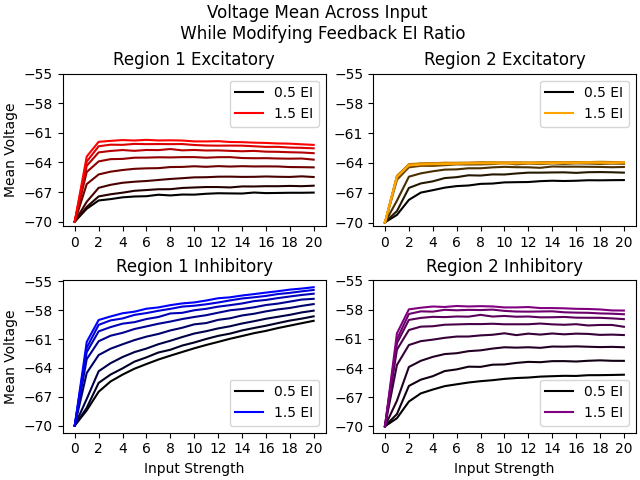
\includegraphics[scale=.8]{twoRegion/EIRatioVoltageMean.png}
    \caption{Modifying feedback EI ratio with fixed feedforward weights $W_{2E1E} = 1.1, W_{2E1I}=1.1$ and fixed feedback excititatory projection $W_{1E2E} = .5$. Decreasing the EI ratio decreases the mean voltage across the network.}
\end{figure}
\begin{figure}
    \centering
    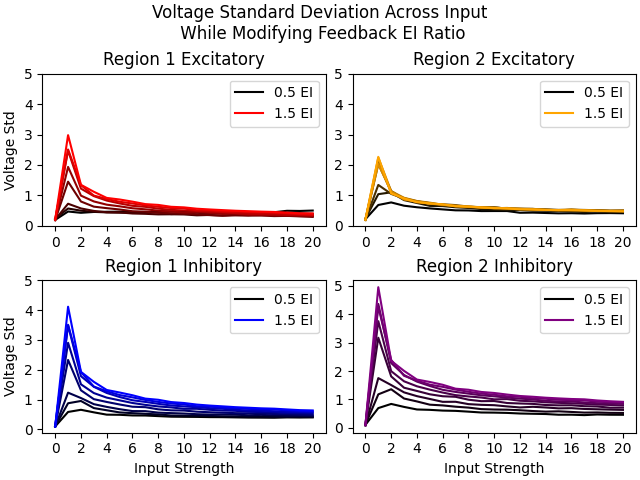
\includegraphics[scale=.8]{twoRegion/EIRatioVoltageStd.png}
    \caption{Modifying feedback EI ratio with fixed feedforward weights $W_{2E1E} = 1.1, W_{2E1I}=1.1$ and fixed feedback excitatory projection $W_{1E2E} = .5$. Lower EI ratio decreases variability across the network.}
\end{figure}
\end{document}
